\section{Introduction}
\label{sec:intro}

\begin{figure*}[!htbp]
\centering
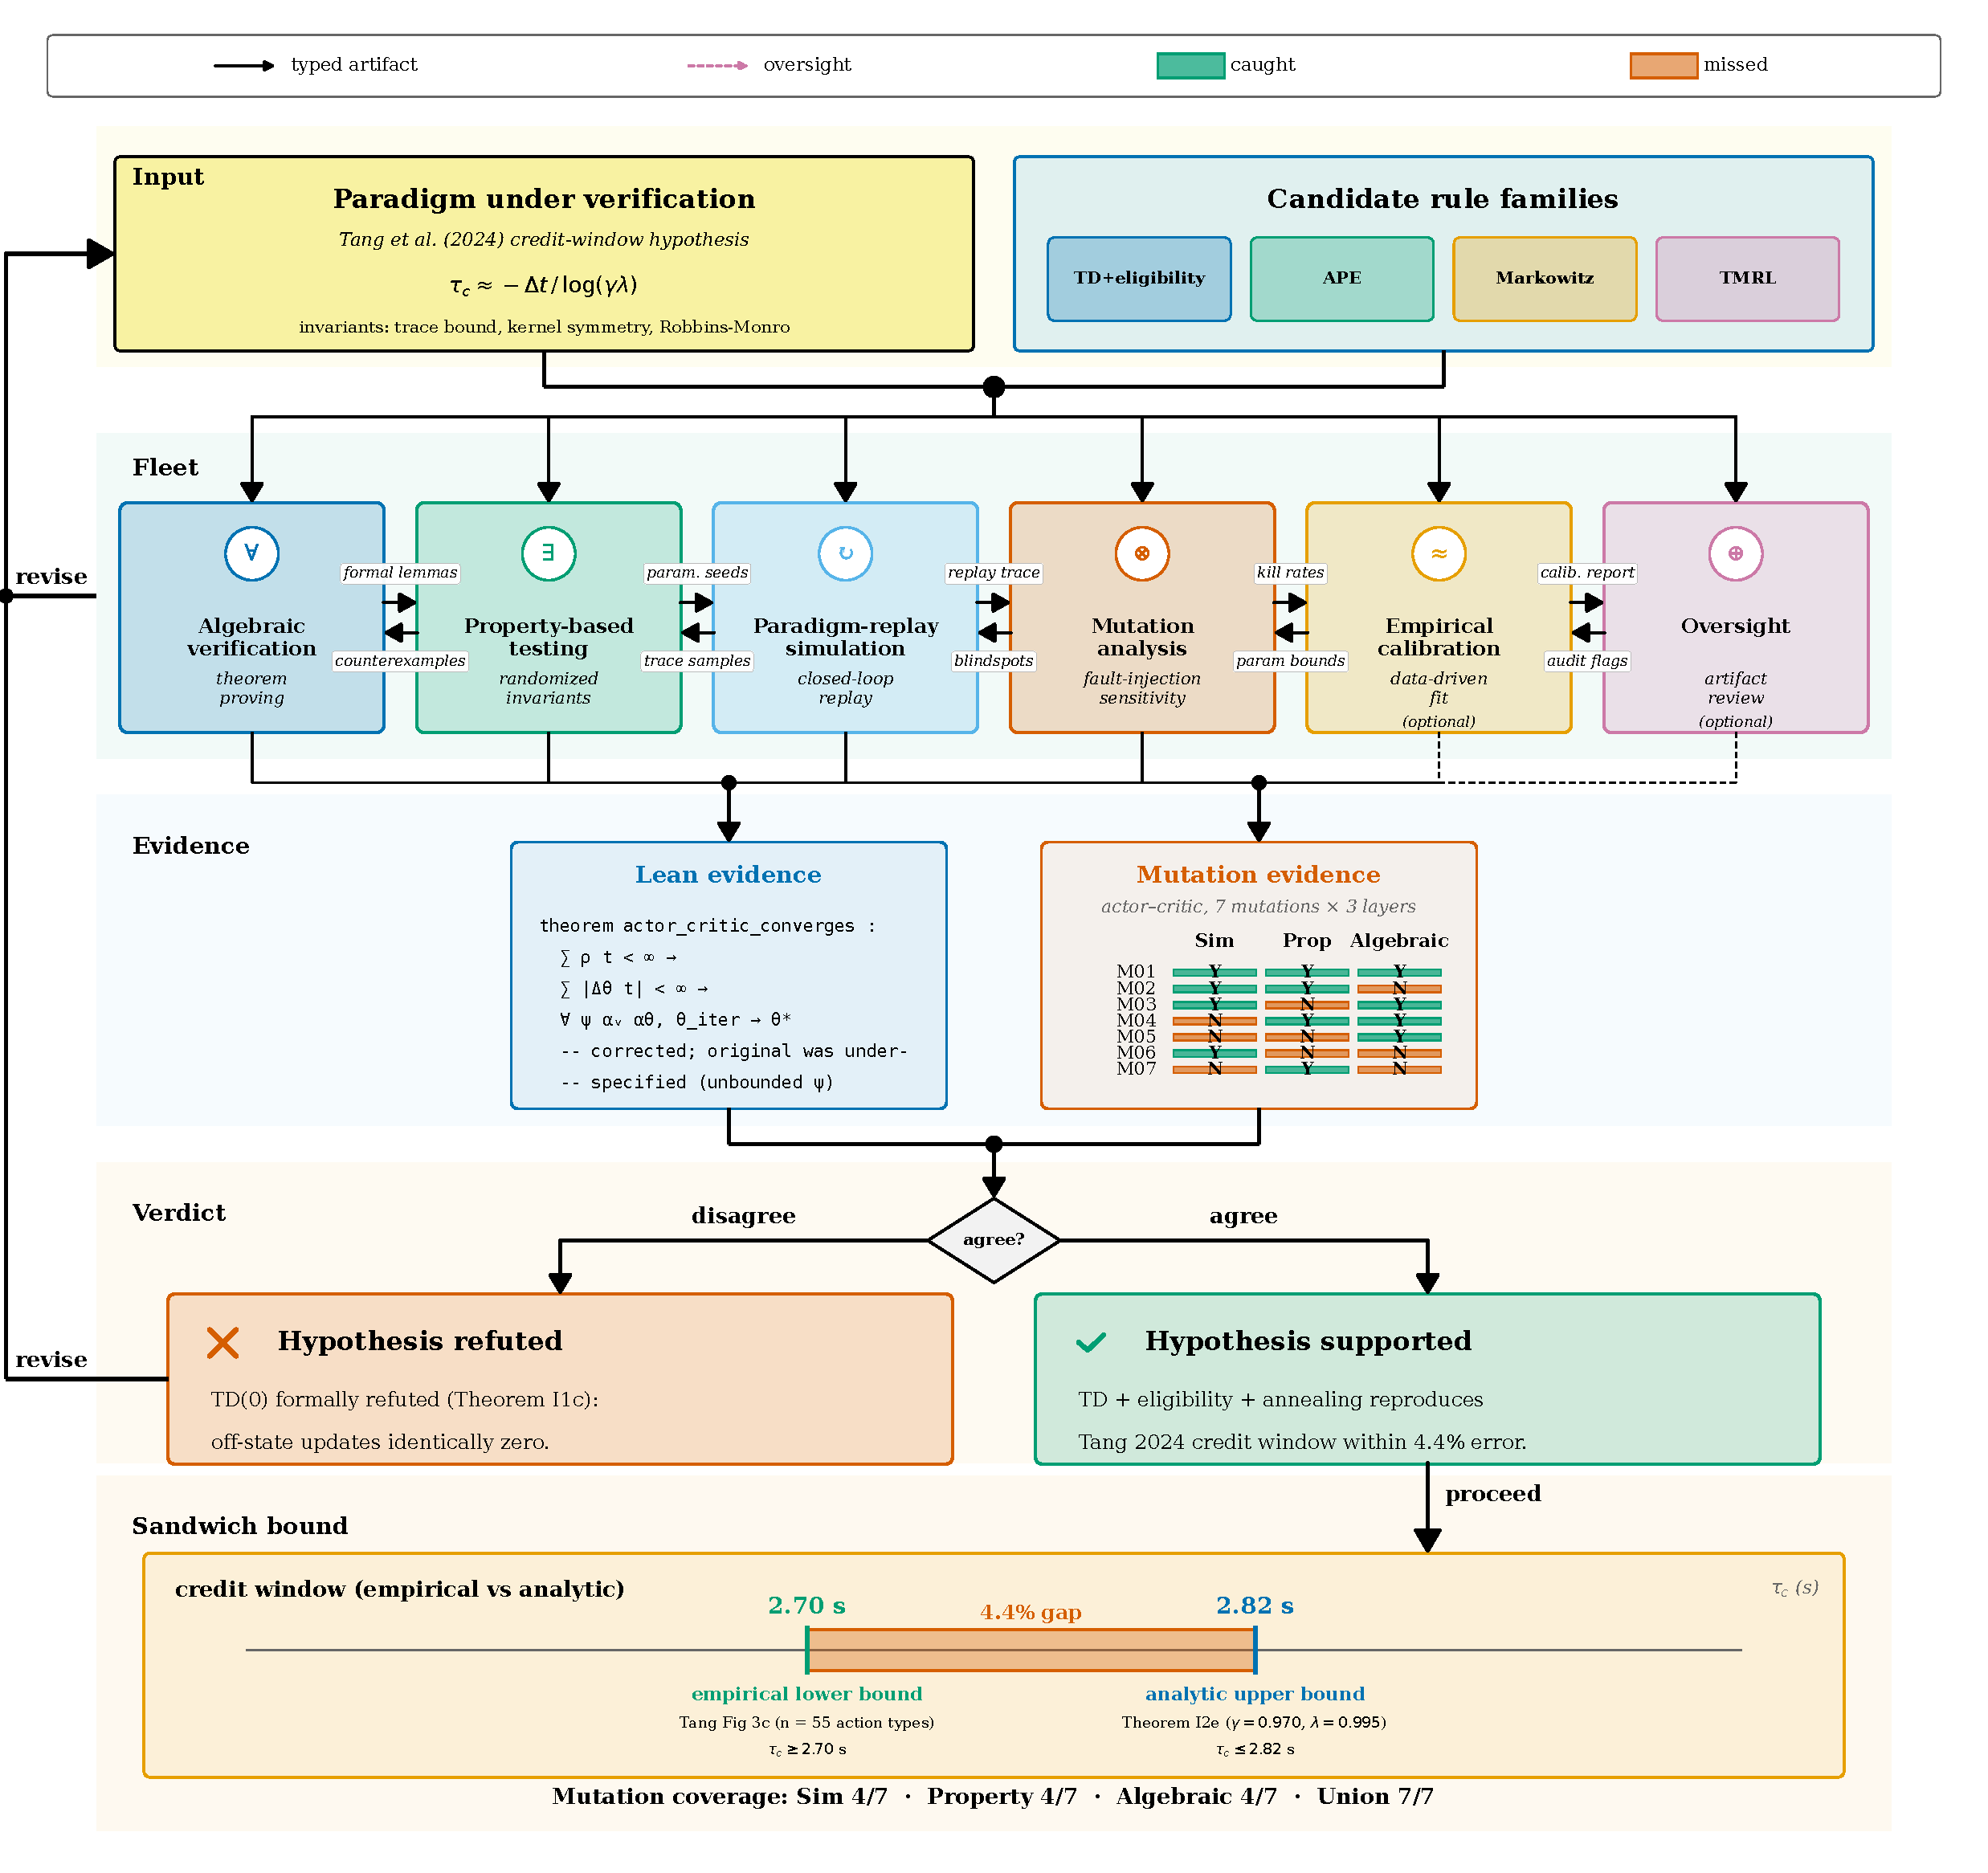
\includegraphics[width=0.90\linewidth]{figures/kairo_pipeline.pdf}
\caption{\textbf{\sys{} decomposes each paradigm claim into six
verification modalities and returns a per-layer verdict with a
sandwich bound.} Four candidate rule families feed six verification
modalities. Refuted claims loop back as revise-hypothesis feedback.
Supported claims flow to the sandwich bound
$\tau_c \in [2.70, 2.82]$\,s (empirical lower, analytic
Theorem~I2e upper, $4.4\%$ gap).}
\label{fig:orchestration}
\end{figure*}

When an animal receives a reward, the brain must determine which
past actions caused it, the credit-assignment
problem~\citep{sutton2018reinforcement}. Computational models
frame this in reinforcement-learning terms: a credit window is
the time over which a reward signal propagates backward, and an
eligibility trace is the decaying weight controlling this
propagation~\citep{singh1996reinforcement}.
Candidate rules inherit convergence guarantees from RL
theorems~\citep{tsitsiklis1997analysis,borkar2000ode}, but those
theorems are rarely re-checked against the form in which they
appear in neuroscience
prose~\citep{schultz1997neural,niv2009reinforcement}. The
actor-critic convergence theorem of
\citet{kondatsitsiklis2000} has been cited for twenty-six years
as the algorithmic account of dopamine-driven
learning~\citep{joel2002actor}. The commonly-retold form drops
an explicit bound on the feature map (Assumption~3.1(a) in the
original). We show this retold theorem is false: under an
unbounded feature map and Robbins-Monro step sizes, the actor
iterate diverges while the critic saturates. A corrected statement
under summability hypotheses machine-checks in
Lean 4~\citep{moura2021lean} with zero unproved obligations and
is strictly stronger than the original.

To produce this result we built \sys{} (Fig.~\ref{fig:orchestration}),
a multi-agent research fleet that checks natural-language scientific
claims against a Lean 4 theorem, property-based
tests~\citep{hypothesis}, and a closed-loop simulation calibrated
on public data~\citep{tang2024dynamic}. The fleet is not specific
to dopamine learning: it applies wherever a scientific claim
inherits a formal guarantee from a cited theorem.

\paragraph{Contributions.}
\begin{enumerate}[leftmargin=1.5em,itemsep=0.1em]
\item \textbf{Formal refutation.} To our knowledge, the first machine-checked
  refutation of a candidate learning rule against an experimental
  feature of a systems-neuroscience paradigm (TD(0) vs.\ the
  Tang et al.\ seconds-scale credit window).
\item \textbf{Corrected theorem.} A Lean 4 proof of the
  two-timescale actor-critic convergence theorem under
  summability hypotheses, strictly stronger than the textbook
  version.
\item \textbf{Per-animal re-analysis.} The reported slow-vs-fast
  learner dichotomy is not bimodal in the eligibility-trace
  parameter $c$. The distribution is continuous ($n=14$).
\item \textbf{Falsifiable prediction.} The analytic credit-window
  bound predicts closed-form the credit-window shift in
  genetically modified mice with reduced dopamine reuptake.
\item \textbf{Agent fleet.} \sys{} as a reusable pipeline for
  formal verification of scientific claims, with verification-gated
  handoffs and persistent shared context across sessions.
\end{enumerate}
